% a-project.tex, v-1.0.3 marcoreis baseado no
% abntex2-modelo-trabalho-academico.tex, v-1.9.7 laurocesar
% Copyright 2012-2018 by abnTeX2 group at http://www.abntex.net.br/ 
% 
% This work consists of the files ........
% 
% -----------------------------------------------------------------------------
% Modelo para desenvolvimento de documentação de projetos acadêmicos
% (tese de doutorado, dissertação de mestrado e trabalhos de monografias em geral) 
% em conformidade com ABNT NBR 14724:2011: Informação e documentação. 
% -----------------------------------------------------------------------------
% Opções para a documentação
%
% Fancy page headings 
%\documentclass[fancyheadings, subook]{Classes/a-prj}
%\documentclass[fancyheadings, sureport]{Classes/a-prj}
%
% Fancy chapters and sections headings 
%\documentclass[fancychapter, subook]{Classes/a-prj}
%\documentclass[fancychapter, sureport]{Classes/a-prj}
%
% Fancy page , chapters and sections headings
%\documentclass[fancyheadings, fancychapter, subook]{Classes/a-prj}
\documentclass[fancyheadings, fancychapter, sureport]{Classes/a-report}
%
% -----------------------------------------------------------------------------
% Alguns comandos para a fancy page headings)
%
% Page header line width
%\footlinewidth{value}
%
% Page footer line width
%\headlinewidth{value}
%
% Page header and footer line width
%\headingslinewidth{value}
%
% Page header and footer lines without text
%\headingslinesonly
%
% The default line width is 0.3pt.
% Set the value to 0pt to remove the page header and/or footer line
%
% -------------------------------------------------------------------------------
% Formato de figuras suportado
% -------------------------------------------------------------------------------
% O formato das figuras depende da forma como o arquivo de saída é gerado.
% As figuras inseridas na pasta Figures serão automaticamente reconhecidas sem
% a necessidade de inserir a extensão do arquivo.
%
% O pdfLaTEX (PDF) suporta figuras com as extensões: pdf, jpg, png e mps.
%
% -------------------------------------------------------------------------------
% Árvore do diretório a-project.tex
%  Diretório
%       \Classes        (requerido)
%       \Figures        (requerido) --------------------------------->
%       \Figures\PDF    (optional)
%       \Figures\JPG    (optional) Figures located within these
%       \Figures\PNG    (optional) folders are searched automatically
%       \Figures\MPS    (optional)  by the a-prj class.
%       \Figures\EPS    (optional)
%       \Figures\PS     (optional) <--------------------------------
%       \Tables         (requerido)
%       \Others         (requerido)
%       \Chapters       (requerido)
%       \Appendices     (optional)
%       \References     (requerido)
%
% -------------------------------------------------------------------------------
% PDF File resumo
\ifpdf
    \hypersetup{
    	backref,
        colorlinks  = true,
        pdftitle    = Modelo de documentação,
        pdfauthor   = {Marco Reis, marco.a.reis@gmail.com},
        pdfsubject  = Mestre em Engenharia,
        pdfcreator  = Subtitulo,
        pdfproducer = PDFLatex,
        pdfkeywords = {documentação, latex, dissertação, tese}}
 \fi
%
% -------------------------------------------------------------------------------
% Relação de pacotes opcionais utilizados
\usepackage[utf8]{inputenc}
\usepackage[brazil]{babel}
\usepackage{longtable}
\usepackage{dcolumn}
\usepackage{multirow}
\usepackage{lscape}
%\usepackage{graphicx}
\usepackage{rotating}
%\usepackage{float,subfigure}
%\usepackage{graphicx, subfigure}
\usepackage{cite}
\usepackage[left=3cm,top=3cm,right=2cm,bottom=2cm]{geometry}
\usepackage[alf]{abntex2cite}
\usepackage{ifpdf}
\usepackage{shadow}
\usepackage{wrapfig}
\usepackage[normalem]{ulem}
\usepackage{makeidx}
\usepackage{yfonts}
\usepackage{algorithm}
\usepackage{algorithmic}
\usepackage{lmodern}
\usepackage[T1]{fontenc}
\usepackage{indentfirst}
\usepackage{color}
\usepackage{microtype}
\usepackage{lipsum}
\usepackage{caption}
\usepackage{subcaption}
\usepackage{listings}

\definecolor{mygreen}{rgb}{0,0.6,0}

\lstset{
  breaklines=true,
  frame=single,
  keepspaces=true,
  commentstyle=\color{mygreen},
  keywordstyle=\color{blue},
  showspaces=false,
  showstringspaces=false,
  showtabs=false,
}

%
\makeindex 
\setlength{\LTcapwidth}{\textwidth}
%
\newtheorem{theorem}{Teorema}
\newtheorem{definition}[theorem]{Definição}
%
% -------------------------------------------------------------------------------
% Configurações do pacote backref
\renewcommand{\backrefpagesname}{Citado na(s) página(s):~}
% Texto padrão antes do número das páginas
\renewcommand{\backref}{}
% Define os textos da citação
\renewcommand*{\backrefalt}[4]{
	\ifcase #1 %
		Nenhuma citação no texto.%
	\or
		Citado na página #2.%
	\else
		Citado #1 vezes nas páginas #2.%
	\fi
}
% 
% -------------------------------------------------------------------------------
% Início do documento raiz
\begin{document}
% Definição do título da página
    \university{Centro Universitário SENAI CIMATEC}
	%\faculty{Programa de...}
	%\school{Escola de...}
% 
    %\course{Engenharia Elétrica}
    \typework{Relatório Final}
% 
	%\course{Mestrado em Modelagem Computacional e Tecnologia Industrial}
	%\typework{Disserta\c{c}\~ao de mestrado}
	%\typework{Exame de Qualificação de Mestrado}
% 
	%\course{Engenharia Elétrica}
	%\typework{Tese de doutorado}
	%\typework{Exame de Qualificação de doutorado}
%
% -------------------------------------------------------------------------------
% Informações gerais
    \thesistitle{Manipulador robótico com visão computacional}
    \hidevolume
    \thesisvolume{Volume 1 of 1}
    \thesisauthor{Tiago Barretto Sant'Anna}
    %\thesisauthorr{Rick Deckard}
    \thesisadvisor{Prof. Marco Reis, M.Eng.}
    %\hidecoadvisor
    %\thesiscoadvisor{Marco Reis}
    \thesismonthyear{Dezembro de 2021}
% 
    \maketitlepage
%
% ----------------------------------------------------------------------------
% Inserir Folha de rosto, Nota de estilo, folha de assinaturas, dedicatoria
    \begin{folharosto}

\begin{center}
\theauthor \\
%\theauthorr \\
%\theauthorrr \\
%\theauthorrrr \\
%\theauthorrrrr \\
\end{center}
\ \\
\ \\
\ \\
\ \\
\ \\
\begin{spacing}{2}
   \begin{center}
   {\LARGE {\bf \thetitle}}
   \end{center}
\end{spacing}
\ \\
\ \\
\ \\
\vspace*{85mm}
% \begin{flushright}

%    \begin{list}{}{
%       \setlength{\leftmargin}{7.5cm}
%       \setlength{\rightmargin}{0cm}
%       \setlength{\labelwidth}{0pt}
%       \setlength{\labelsep}{\leftmargin}}

%       \item \thetypework apresentada ao \thefaculty, Curso de \thecourse
%       do \theuniversity, como requisito parcial para a obten\c{c}\~ao do
%       t\'itulo de {\bf \thedegreetitle}.

%       \begin{list}{}{
%       \setlength{\leftmargin}{0cm}
%       \setlength{\rightmargin}{0cm}
%       \setlength{\labelwidth}{0pt}
%       \setlength{\labelsep}{\leftmargin}}

%       \item \'Area de conhecimento: Interdisciplinar

%       \item Orientador: \theadvisor
%       \newline \hspace*{2.1cm}  %{\it \theuniversity}

%       \end{list}
%    \end{list}

% \end{flushright}
\ \\
\ \\
\ \\
\ \\
%\begin{spacing}{1.5}
   \begin{center}
   Salvador \par
   \theuniversity \par
   2020
   \end{center}
%\end{spacing}

\end{folharosto}

    %\begin{notaestilo}
Esta \thetypeworkthree foi elaborada considerando as normas de
estilo (i.e. est\'eticas e estruturais) propostas aprovadas pelo
colegiado do \thefacultytwo e est\~ao dispon\'iveis em formato
eletr\^onico ({\it download} na P\'agina Web
http:$//$ead.fieb.org.br$/$portal\_faculdades$/$dissertacoes-e-teses-mcti.html
ou solicita\c{c}\~ao via e-mail \`a secretaria do
programa) e em formato impresso somente para consulta. \\

Ressalta-se que o formato proposto considera diversos itens das
normas da Associa\c{c}\~ao Brasileira de Normas T\'ecnicas (ABNT),
entretanto opta-se, em alguns aspectos, seguir um estilo pr\'oprio
elaborado e amadurecido pelos professores do programa de
p\'os-gradua\c{c}\~ao supracitado.

\end{notaestilo}

    %\begin{folhaassinaturas}

%\thispagestyle{empty}

\def\signature#1#2{\parbox[b]{1in}{\smash{#1}\vskip12pt}
\hfill \parbox[t]{3in}{\shortstack{\vrule width 3in height
0.4pt\\\small#2}}}

\def\InstituicaoMembro#1#2{\parbox[b]{1in}{\smash{#1}\vskip12pt}
\hfill \parbox[t]{3in}{\shortstack{\vrule width 3in \\\small#2}}}

\def\signaturepage{%

    \begin{spacing}{1.5}
        \begin{center}
        {\LARGE \theuniversity} \\
        {\large \thefaculty} \\
        {\large \thecourse} \\
        \end{center}
    \end{spacing}

   \vskip 0.25in plus 0.4in minus 0.1in

    \begin{spacing}{1.5}
        \begin{sloppypar}
        A Banca Examinadora, constitu\'ida pelos professores abaixo
        listados, leram e recomendam a aprova\c{c}\~ao [com distin\c{c}\~ao] da
        \thetypeworktwo, intitulada ``\thetitle",
        apresentada no dia (dia) de (m\^es) de (ano), como requisito
        parcial para a obten\c{c}\~ao do t\'itulo de {\bf \thedegreetitle}.\\
        \end{sloppypar}
    \end{spacing}

    \def\sigskip{\vskip0.15in plus 0.2in minus 0.1in}
    \def\beginskip{\vskip0.3875in plus 0.2in minus 0.1in}

    \beginskip
    \signature{Orientador:}{Prof. Dr. \theadvisor} \\
    \InstituicaoMembro{}{\theuniversity} \\

    \sigskip
    \beginskip
    \signature{Membro externo da Banca:}{Prof. Dr. Nome completo} \\
    \InstituicaoMembro{}{Institui\c{c}\~ao do membro da banca} \\

    \sigskip
    \beginskip
    \signature{Membro externo da Banca:}{Prof. Dr. Nome completo} \\
    \InstituicaoMembro{}{Institui\c{c}\~ao do membro da banca} \\

    %\sigskip
    %\beginskip
   % \signature{Membro interno da Banca:}{Prof. Dr. Nome completo} \\
   % \InstituicaoMembro{}{Institui��o do membro da banca} \\

    \vfill
    \newpage
    \setcounter{page}{3}
}
%*********************************************************************


\signaturepage


\end{folhaassinaturas}

    %\include{Others/dedicatoria}
    %\include{Others/agradecimentos}
%
% ----------------------------------------------------------------------------
% Resumo/abstract, sumário e siglas
    % \begin{romanpagenumbers}
    %     \begin{thesisresumo}



\textbf{Palavras-chave}: robótica, estudo, programação, simulação.

\end{thesisresumo}

    %     \begin{thesisabastract}
    The work consists in the explanation of the perceptions about the established challenges. So this report shows how it was developed and the tactics used to complete this activity. It aims to absorb knowledge in order to carry out robotics projects. For this, several studies were carried out to be able to carry out these challenges.

%Escreva aqui, em ingl\^es, o resumo da disserta\c{c}\~ao, incluindo os contextos geral e espec\'ifico, dentro dos quais a pesquisa foi realizada, o objetivo da pesquisa, assun\c{c}\~ao filos\'ofica, os m\'etodos de pesquisa usados e as poss\'iveis contribui\c{c}\~oes que o que \'e proposto pode trazer \`a sociedade. 

\ \\

% use de tr�s a cinco palavras-chave

\textbf{Keywords}: robotics, study, programming, simulation.

\end{thesisabastract}

    %     % Make list of contents, tables and figures
    %     \thesiscontents
    %     %\pdfbookmark[1]{Lista de Tabelas}{lot} \listoftables
    %     \newpage
    %     %Include other required section
    %     %\begin{thesisabbreviations}
\begin{footnotesize}
\begin{longtable}[l]{p{2cm}l}
  tprax   \dotfill & \thefaculty \\
  WWW       \dotfill &  World Wide Web \\
\end{longtable}
\end{footnotesize}
\end{thesisabbreviations}

    %     %\begin{thesissymbols}
\begin{footnotesize}
\begin{longtable}[l]{p{2cm}l}
  $\partial$   \dotfill  & Bla bla bla \\
  $\prod$       \dotfill & ble ble ble \\
  $\partial$   \dotfill  & Bla bla bla \\
  $\prod$       \dotfill & ble ble ble \\
  $\partial$   \dotfill  & Bla bla bla \\
  $\prod$       \dotfill & ble ble ble \\
  $\partial$   \dotfill  & Bla bla bla \\
  $\prod$       \dotfill & ble ble ble \\
  $\partial$   \dotfill  & Bla bla bla \\
  $\prod$       \dotfill & ble ble ble \\
  $\partial$   \dotfill  & Bla bla bla \\
  $\prod$       \dotfill & ble ble ble \\
  $\partial$   \dotfill  & Bla bla bla \\
  $\prod$       \dotfill & ble ble ble \\
  $\partial$   \dotfill  & Bla bla bla \\
  $\prod$       \dotfill & ble ble ble \\
  $\partial$   \dotfill  & Bla bla bla \\
  $\prod$       \dotfill & ble ble ble \\
  $\partial$   \dotfill  & Bla bla bla \\
  $\prod$       \dotfill & ble ble ble \\
  $\partial$   \dotfill  & Bla bla bla \\
  $\prod$       \dotfill & ble ble ble \\
  $\partial$   \dotfill  & Bla bla bla \\
  $\prod$       \dotfill & ble ble ble \\
  $\partial$   \dotfill  & Bla bla bla \\
  $\prod$       \dotfill & ble ble ble \\
  $\partial$   \dotfill  & Bla bla bla \\
  $\prod$       \dotfill & ble ble ble \\
  $\partial$   \dotfill  & Bla bla bla \\
  $\prod$       \dotfill & ble ble ble \\
  $\partial$   \dotfill  & Bla bla bla \\
  $\prod$       \dotfill & ble ble ble \\
  $\partial$   \dotfill  & Bla bla bla \\
  $\prod$       \dotfill & ble ble ble \\
  $\partial$   \dotfill  & Bla bla bla \\
  $\prod$       \dotfill & ble ble ble \\
  $\partial$   \dotfill  & Bla bla bla \\
  $\prod$       \dotfill & ble ble ble \\          
\end{longtable}
\end{footnotesize}
\end{thesissymbols}

    %     %Switch the page numbering back to the default format
    % \end{romanpagenumbers}
%
% ---------------------------------------------------------------------------
% Include thesis chapters
    \parskip=\baselineskip
    \chapter{Introdução}
\label{chap:intro}




%--------- NEW SECTION ----------------------
\section{Objetivos}
\label{sec:obj}
Os objetivos são realizar a programação de um manipulador robótico especializado, em conjunto com visão computacional para poder realizar a automação de tarefas.
\label{sec:obj}

\subsection{Objetivos Específicos}
\label{ssec:objesp}
Os objetivos específicos deste projeto são:
\begin{itemize}
      \item Controlar um manipulador utilizando o ROS
      \item Identificar Objetos utilizando visão computacional
      \item Integrar o manipulador com a visão computacional
  \end{itemize}

%\subsubsection*{Objetivos específicos principais}
%\label{sssec:obj-principais}


%--------- NEW SECTION ----------------------
\section{Justificativa}
\label{sec:justi}

Justificativa

%--------- NEW SECTION ----------------------
\section{Organização do documento}
\label{section:organizacao}

Este documento apresenta $3$ capítulos e está estruturado da seguinte forma:

\begin{itemize}

  \item \textbf{Capítulo \ref{chap:intro} - Introdução}: Contextualiza o âmbito, no qual a pesquisa proposta está inserida. Apresenta, portanto, a definição do problema, objetivos e justificativas da pesquisa e como este \thetypeworkthree está estruturado;
  \item \textbf{Capítulo \ref{chap:08-02-22} - Dia: XX/XX/XX}: Explicita com toda a base teorica como o trabalho foi desenvolvido diariamente, o processo para a sua obtenção.

\end{itemize}

    \chapter{Dia: 09/02/22}
\label{chap:09-02-22}
    \chapter{Dia: 09/02/22}
\label{chap:09-02-22}

Primeiro surgiu uma tentativa de testes do dobot usando a docker porém o seguinte erro aparecia no terminal:

\begin{figure}[h!]
    \centering
    \caption{terminal}
    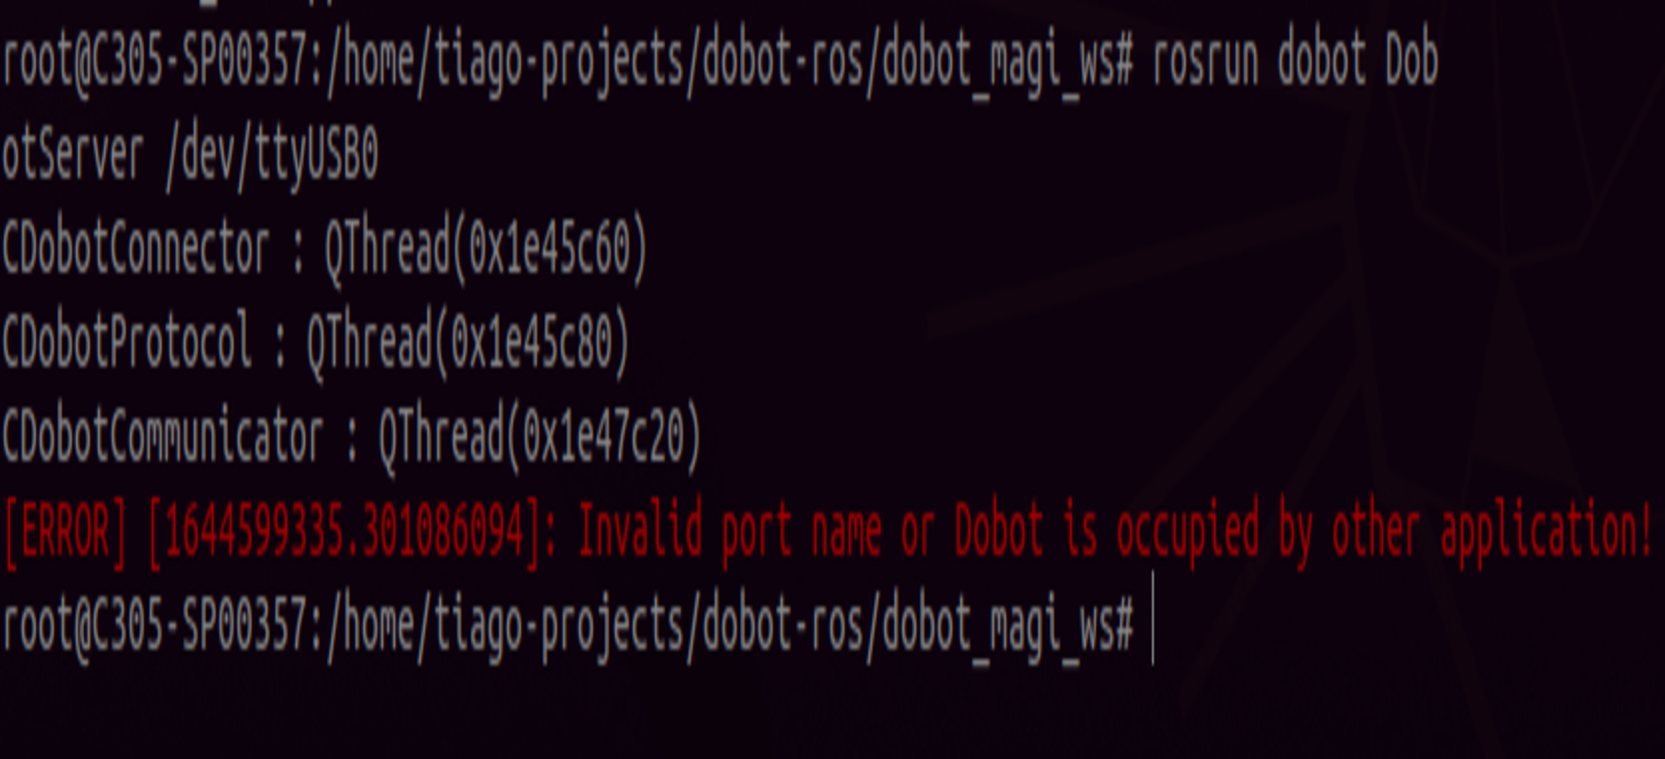
\includegraphics[width=1\textwidth]{Figures/dob1.jpg}
    \caption*{Fonte: Autoria propria.}
    \label{fig:teminal1}
\end{figure}

A primeira hipótese foi substituir a docker que estava sendo utilizada, que era uma docker de ROS Kinetic, e retorna para o tipo de docker que estava sendo utilizada anteriormente, que era uma docker de ubuntu xenial com ubuntu instalado. Isso foi feito com base no fato de que na primeira tentiva se tinha usado a docker dessa forma e tinha funcionado, precisaria de um OS para poder controlar as portas e no manual está recomendado o uso dessa versão do ubuntu com essa versão do ros instalado. A partir disso foi criado essa imagem do xenial com o ROS Kinetic instalado e armazenado no seguinte repositório no \href{https://hub.docker.com/repository/docker/tiago369/ubuntu-kinect}{DockerHUB}.

Porém, mesmo realizando isso o problema persistiu e decidiu investigar mais ainda o uso de portas USB na docker, a partir disso descobriu-se que precisava subir as portas USBs que seriam utilizadas, assim no código de docker\underline{\space}run\underline{\space}xenial.sh foi substituído a parte que sobe as portas de videos pela USB

Antes:

\begin{lstlisting}[language=Awk]
    V4L2_DEVICES=" "

    for i in {0..9}
    do
        if [ -a "/dev/ttyVideo$i" ]; then
            V4L2_DEVICES="$V4L2_DEVICES --device /dev/ttyVideo$i "
        fi
    done

    echo "V4L2_DEVICES:  $V4L2_DEVICES"
\end{lstlisting}

Depois:

\begin{lstlisting}[language=Awk]
    V4L2_DEVICES=" "

    for i in {0..9}
    do
        if [ -a "/dev/ttyUSB$i" ]; then
            V4L2_DEVICES="$V4L2_DEVICES --device /dev/ttyUSB$i "
        fi
    done

    echo "V4L2_DEVICES:  $V4L2_DEVICES"
\end{lstlisting}

Depois disso o DOBOT conseguiu se conectar e se partiu para o desenvolvimento dos códigos
    \chapter{Dia: 10/02/22}
\label{chap:10-02-22}

Nesse dia foi majoritariamente focado no do desenvolvimento da programação para o funcionamento do Dobot.

A demo do DOBOT funciona utilizando Services e o \cite{Dobotand76:online} fez um tópico para poder movimentar o braço. Assim o primeiro desafio foi aprender a utilizar os Services do ROS, para isso foi utilizado a própria wiki oficial \cite{rospyOve3:online}.

\begin{lstlisting}[language=Python]
    #!/usr/bin/env python
    import rospy

    from dobot.srv import GetPose

    if __name__ == '__main__':
        print('1')
        # rospy.wait_for_service('print_pose')
        get_pose = rospy.ServiceProxy('DobotServer/GetPose', GetPose)
        print('2')


        try:
            print('a')
            print(get_pose())
            print('b')
        except rospy.ServiceException as exc:
            print("Service did not process request: " + str(exc))

        var = get_pose()
        print(var.x)
\end{lstlisting}

Dessa forma foi desenvolvido um código para poder exibir na tela a posição atual, já que seria necessário receber a posição do braço para poder fazer os cálculos da sua movimentação. Assim após finalizado foram incrementados no código position\underline{\space}control.py para controle de posição desenvolvido esse services

\begin{lstlisting}[language=Python]
    #!/usr/bin/env python
    from turtle import pu
    import rospy
    from geometry_msgs.msg import Pose
    import time
    from dobot.srv import GetPose
    import math

    def distancia(ini, fim):
        return math.sqrt((fim - math.sqrt((ini)**2))**2)

    def position():
        rospy.init_node('position_control', anonymous=True)
        publisher = rospy.Publisher('geometry_pose', Pose, queue_size=10)
        get_pose = rospy.ServiceProxy('DobotServer/GetPose', GetPose)


        print("Say where you want me to go")
        x = int(input("X axis: "))
        y = int(input("Y axis: "))
        z = int(input("Z axis: "))

        freq = rospy.Rate(0.5)
        dist = 1

        k = 10

        while dist >= 0.1:
            print('a')
            msg = Pose()
            pose = get_pose()
            
            msg.position.x = k * distancia(pose.x, x)
            msg.position.y = k * distancia(pose.y, y)
            msg.position.z = k * distancia(pose.z, z)
            publisher.publish(msg)

            dist = (distancia(pose.x, x) + distancia(pose.z, z) + distancia(pose.y, y)) / 3

            freq.sleep()

    if __name__ == "__main__":
        try:
            position()
        except rospy.ROSInterruptException:
            pass
\end{lstlisting}

Esse código foi feito baseado no código desenvolvido por \cite{Dobotand76:online}. Porém, nenhuma das suas versões conseguiram movimentar o braço robótico.

    \chapter{Dia: 11/02/22}
\label{chap:11-02-22}

Foi corrigido o código do pick\underline{\space}and\underline{\space}place.py o DOBOT conseguiu se mover como mostrado no video seguinte: \href{https://youtu.be/nkaut31VhHA}{Dobot} 
Porém a bomba ainda continua soprando ar ao invés de puxar e o braço ainda continua com o movimento muito lento

    % \include{Chapters/}
    % \include{Chapters/Desenvolvimento}
%    \include{Chapters/fundamentos}
%    \include{Chapters/metodos}
%    \include{Chapters/resultados}
    % \include{Chapters/conclusao}
    % include more chapters ...
%
% ----------------------------------------------------------------------------
% % Include thesis appendices
%     \begin{thesisappendices}
%         % % Thesis Appendix -------------------------------------------------------

\chapter{Diagramas mecânicos}
\label{Append:diagmec}



%         % % Thesis Appendix -------------------------------------------------------

\chapter{Diagramas eletro-eletrônicos}
\label{Append:diagele}



%         %% Thesis Appendix -------------------------------------------------------

\chapter{Logbook}
\label{Append:log}



%     \end{thesisappendices}
%
% ----------------------------------------------------------------------------
% Configurar as referencias bibliograficas
	\renewcommand\bibname{Referências}
    \addcontentsline{toc}{chapter}{Referências}
    \bibliography{References/referencias}
%
% ----------------------------------------------------------------------------
% Finishing him
    \include{Others/ultimafolha}
\end{document}
%
% -------------------------------------------------------------------------------
% Aqui termina a formatação para o documento.
% In God We Trust. All Other Bring Data. 
%
% -------------------------------------------------------------------------------